\documentclass[WHATMANUAL.tex]{subfiles}

\begin{document}

\chapter{Estimation of missing daily climatological data}\label{chap:Missing_weather_theory}

\section{Introduction}

Climate data are useful in several fields of Earth Sciences, including hydrology, hydrogeology and agronomy. However, climate datasets are often incomplete. This represents a serious issue to the use of models that depend on these data. For example, the method used for the estimation of groundwater recharge in WHAT requires serially complete (no missing data values) air temperature and precipitation daily time series. The quality of the groundwater recharge assessments made with this technique are highly dependent upon the quality of the weather date set used. Hence, the adequate and accurate handling of missing data has been made an integral part of groundwater recharge assessment in WHAT.

A guide for the preparation of gapless weather data series has already been presented in Section~\ref{chap:gapfilling}. This section presents a brief literature review on the subject, followed by a detailed description of the method implemented in WHAT for the estimation of missing daily weather data, and finally an application is presented for the Monteregie Est region, located in southern Quebec, Canada. 

\section{Literature review}

Filling the gaps in weather data time series is a tedious task that can become rather complex when efficiency of the method, accuracy in the estimation of the missing values, and preservation of the statistical properties of the weather time series (probability distribution and normals) are required. This is particularly true for the estimation of missing daily precipitation data because of their high spatial and temporal variability \citep{simolo_improving_2010}. 

The creation of a serially complete weather dataset generally consists in the replacement of missing daily data with estimated values calculated from simultaneous observations at nearby stations. Within-station method, i.e. methods that only use data from the series being filled, have been proven to perform badly compared to methods based on the use of data from neighboring stations and are moreover ill-adapted for the reconstruction of daily precipitation time series \citep{eischeid_quality_1995,simolo_improving_2010,kemp_estimating_1983}.

Numerous spatial interpolation techniques exist for handling the missing data in the weather time series of a given station by using data from irregularly spaced neighboring station (e.g. simple arithmetic averaging, inverse distance method, single best estimator and multiple regression analysis). \cite{eischeid_creating_2000} demonstrated that the multi-linear regression (MLR) method \citep{degaetano_method_1995} outperformed most of the commonly used techniques among the six classical methods tested for the creation of a serially complete daily temperature and precipitation dataset for the United States. Similarly, \cite{xia_forest_1999} also found that the MLR method was consistently the most accurate out of the six classical methods tested to estimate missing daily weather data in Bavaria, Germany. One of the advantage the MLR approach has over many classical method is that it can account for the local effect (i.e. topography, land cover, land use, surface water).

However, weighing and regression-based techniques, including the MLR method mentioned above, all tend to overestimate the number of rainy days. Also, the rainfall probability distribution is usually not preserved with these techniques, that is heavy precipitation events are systematically underestimated. \cite{simolo_improving_2010} have proposed a two-step procedure to modifies the MLR method to address these issues.

In recent years, the estimation of missing daily weather data using artificial intelligence techniques have been the subject of many research studies \cite{kashani_evaluation_2011,kim_spatial_2008,srikanthan_comparison_2005,coulibaly_comparison_2007,abebe_application_2000,teegavarapu_improved_2005}. \cite{kashani_evaluation_2011} found that these new data-driven methods, more specifically the artificial neural network and the genetic programming techniques, outperformed the classical application of the MLR approach for three different climates in Iran. Artificial intelligence techniques are interesting because, unlike the classical weighing and regression-based methods, they are able to reflect the inherently stochastic nature of natural processes. Nevertheless, the results of \cite{kashani_evaluation_2011} also indicated that the MLR method was an appropriate technique, among the eight traditional methods tested, for all the weather variables (air temperature, wind speed, relative humidity, and precipitation) and the different climate conditions (dry to extra humid conditions) tested \citep{kashani_evaluation_2011}.

\section{Description of the method}

Though there exist various methods to estimate missing daily weather data that are well covered in textbooks and technical papers, tools to perform this task quickly, efficiently and easily are scarce. The implementation of some of the more complex (and often most accurate) methods discussed in the section above can be a daunting task for a research study that is not directly related to the fields of meteorology or to the geostatistics. Because of time or resources constraints, it can be tempting in these studies to handle the problem of missing daily weather data with a simple method that is not always appropriate to the objective of the study. This is the case for example of using a simple and practical within-station approach to quickly and easily estimate missing values for daily air temperature and precipitation which is not an appropriate method for these kind of data \citep{eischeid_quality_1995,simolo_improving_2010,kemp_estimating_1983}. For this reason, the creation of gapless weather data series (air temperature and precipitation) has been made an integral part of the software WHAT.

The method for filling the gaps in the weather time series of air temperature and precipitation is based on the implementation of the classical MLR method presented in \cite{eischeid_creating_2000}. The rationales behind this choice was to provide in WHAT a robust, efficient, accurate, and well known method that was adequate to most conditions (e.g. climate, land cover, topography). Based on the literature review presented in the section above, this choice appears to be a very good default option for the first a version of the software. Since the code for loading and manipulating the entire weather dataset of a given study area is object oriented, it should be relatively easy to add modifications to the currently available approach such as the additional steps for the MLR method proposed in \cite{simolo_improving_2010} or to completely implement one of the new artificial intelligence techniques that were developed in recent years \citep{kashani_evaluation_2011}.

In addition to the handling of missing data, WHAT includes the framework to easily validate and assess the uncertainty of the estimated missing values with a jackknife resampling technique. This feature is an invaluable tool for quickly validating the method for a given study area and to test the performance of new methods that could be added to future version of the software. The entire gapfilling process used in WHAT is illustrated in the flowchart of Figure~X.

\begin{figure}
\centering

\includegraphics[height=0.95\textheight]{img/Flowchart-filling_missing_weather}
\caption[WHAT workflow.]{WHAT workflow for the interpretation of groundwater-level time-series measured in an observation well or a piezometer.}
\label{fig:flowchart_GapFilling}
\end{figure}

\subsection{Step 1: Pre-processing}

\subsubsection{Quality Check}

Prior to the analysis of climatic time series, it is important to do some consistency checks to ensure that the data do not violate obvious constraints associated with minimum, maximum, and average daily air temperature and daily cumulative precipitation. This step is not included in the gap filling routine per se. It is why it does not appear in the flowchart of Figure~\ref{fig:flowchart_GapFilling}. It is done every times the software scans the ``Input''folder for new weather data file and load them into memory (see Section~\label{guide-gapfilling}).

The program will check to insure that maximum, minimum and average daily temperature are coherent for a given day. It also check that all daily cumulative precipitation values are positive.

When inconsistencies are detected, the program emit a warning and offer the choice to replace these wrong values with a ``NaN'', so that they can be properly estimated by the program from neighboring stations.

\subsubsection{Station Correlation Assessment}

The subsequent step consists in calculating the correlation coefficients between data of the target station and those of the neighboring stations for each of the four weather variables: minimum, maximum and average daily temperature and daily cummulative precipitation. The calculation of the coefficients are done for the entire time-series for each neighboring station individually. If there is less than 182 synchronous values between the data of the target station and those of a neighboring station for a given variable, the correlation is not computed and a ``NaN'' value is kept instead.

An alternative approach would have been to calculate the correlation coefficient with a subsets of data from the target series centered around the missing value, as it was done in \cite{simolo_improving_2010}, for example. This approach allows to better represent the seasonal variations in the relations between the stations. The downsides include a more complex algorithm to implement and a reduction of the method robustness and efficiency. This alternative should however be added as an additional option in a future version of WHAT and its impact on the accuracy of the method should be assessed.

Based on our experience with daily weather data in Canada, the correlation coefficients between time-series of air temperature measurements is generally higher than 0.98 for stations located at a distance of 100~km or less. The relation between the station precipitation is much more sensitive to variations in the landscape (land cover, topography, surface water). As a result, correlation coefficients are generally less than for air temperature and decrease more rapidly with the distance from the target station. A value higher than 0.8 is generally acceptable.

In addition to the correlation coefficient, the horizontal and vertical distances between the target and the neighboring stations are calculated. Data correlation between two stations will generally decreases as the horizontal and vertical distances increase. It is possible to specify a cutoff distance and a cutoff altitude difference for which neighboring stations that fall above these cutoff values are ignored by the program. The default values are set to 100~km and 350~m for the horizontal and vertical distance respectively based on the literature 
\citep{tronci_comparison_1986,xia_forest_1999,simolo_improving_2010}.

\subsection{Step 2: Filling the Gaps}

The procedure for filling the gaps in the weather data includes two nested loops. The external loop, labeled ``Loop A'' in Figure~\ref{fig:flowchart_GapFilling}, iterates over the time series of four weather variables for the target station. The inner loop, labeled ``Loop B'', iterates over every missing values in the data series. The process for the estimation of a single missing value is basically a two step procedure. The first step consists in selecting the data series with the best corellation coefficient. The second step consiste in building a MLR model and estimate the missing values. This is described in more details in the following text.

\subsubsection{Selection of the neighboring stations}

The selection of surrounding stations is critically important for accurate estimation of missing weather data \citep{eischeid_quality_1995}. Problems arise though because of synchronized missing values in the target and neighboring weather station data series that varies trough time. This is illustrated in Table~\ref{tab:example_selectStations} where are presented theoretical time-series of air temperature data with a realistic distribution of missing values.

\begin{table}[!hb]
\newcommand{\nan}{\multicolumn{1}{c}{\textbf{nan}}}
\newcolumntype{d}{D{.}{.}{2.1} } %decimal column as before
\center
\caption{This table shows some data}
\begin{tabular}{*6{d}}
\toprule
\multicolumn{1}{c}{} &
\multicolumn{1}{c}{Target} &
\multicolumn{4}{c}{Neighbors} \\
\cmidrule(r){3-6}
\multicolumn{1}{c}{Day}&
\multicolumn{1}{c}{X}  &
\multicolumn{1}{c}{Y1} &
\multicolumn{1}{c}{Y2} &
\multicolumn{1}{c}{Y3} &
\multicolumn{1}{c}{Y4}\\
\midrule
%\rowcolor{gray!30}
1 & 11.0 & 12.0 & 12.0 & 12.5 & 10.0 \\
2 & \nan & 12.0 & \nan & 13.0 & 12.2 \\
3 &  7.5 &  8.5 &  8.5 &  8.0 &  8.9 \\
4 & \nan &  6.0 &  4.5 &  5.0 &  4.4 \\
5 & \nan &  8.0 &  8.5 & \nan & \nan \\
% 6 & 5.0  & 8.5  & 5.0  &  6.5 &  4.4 \\
% 7 & 15.0 & 17.0 & 15.0 & 15.5 &  8.9 \\
% 8 & 13.5 & 16.0 & 11.0 & 15.0 &  4.4 \\
% 9 & 11.5 & 13.0 & 12.5 & 10.0 & 15.6 \\
%10 & 15.5 & 19.0 & 19.5 & 18.0 & 16.1 \\
\bottomrule
\end{tabular}
\label{tab:example_selectStations}
\end{table}

There is missing values in the target station data series at days 2, 3, and 5. The missing value on day 2 will be estimated with the data of the neighboring stations Y1, Y3, and Y4 since station Y2 is also missing a value at this time. All neighboring stations will be used for the estimation of the missing value on day 4 while only stations Y1 and Y2 have data available for the estimation of the missing value on day 5.

Since the number of neighboring stations with available data is not fixed in time, it is not possible to use a single MLR model to fill all the missing values for the target station all at once. 
 
For each missing value in the series of the target station, the program keeps only the data series of the neighboring stations that also have data at this particular time. Data series of stations not respecting the distance and cutoff criteria are also ignored. The data from the neighboring stations are then selected in descending order of their correlation coefficient with the target station, up to a maximal number of station defined in the method parameters. The default value for the maximal number of neighboring station is four based on the literature \citep{eischeid_quality_1995,xia_forest_1999}.

If for a given day all the neighboring stations have missing values synchronously with the target station, no estimation is being done and a ``nan'' value is kept in the series instead and the program pass to the next missing value in the target series.

\subsubsection{Multiple Linear Regression Model}

First the program will check if the sequence of neighboring stations has already been encountered for the current weather variable and will load the MLR parameters from memory if this is the case and will directly estimate the missing value. Otherwise, the model will generate a new MLR model using either an Ordinary Least Square (OLS) or a Least Absolute Deviations (LAD) criteria (bot options are available in the method).

Since daily cumulative precipitation are generally represented by long-tailed distributions that are positively skewed, the LAD criteria is a better option than the OLS criteria for handling these kind of dirstribution because it is more robust to outliers \citep{eischeid_quality_1995,eischeid_creating_2000}. The downside is an increase in computation time. The MLR using a LAD criteria is computed in WHAT with a iterative reweighted least squares method \citep{schlossmacher_iterative_1973}.  \citep{eischeid_quality_1995}. 
 
\subsubsection{Estimating Missing Daily Value}

When the parameters of the MLR model for a given day with a missing value are known, the missing value in the target time series is estimated as:

\begin{equation}
    X(t) = a_0 + \sum_{i=1}^{N} a_i \cdot Y_i(t)
\end{equation}

where $a_i$ are the regression coefficients, $X(t)$ is the missing value of the target station estimated at time $t$, $Y_i$ are the synchronous values of the neighboring stations, and $N$ is the total number of neighboring stations used for the regression, up to the maximal value defined in the method (default is four).

When all missing values in the target station dataset have been estimated, the resulting gap free time series is saved in a ``.out'' file. Detailed information about the estimated values are saved in an accompanying ``.log'' file (see Section~\ref{guide-gapfilling}).

\subsection{Step 3: Validation}

WHAT also includes an option to perform a validation of the method used for a particular weather dataset with a jackknife procedure. This option is an advanced feature that can be activated by changing the value of the field ``Full Error Analysis'' from 0 to 1 in the file named ``WHAT.pref'' (see Section~\ref{guide-gapfilling}).

More specifically, when this option is activated, WHAT will estimate a value for the target station for every day of the time series. In other words, the loop B in the flowchart of Figure~\ref{fig:flowchart_GapFilling} will run over all the days of the data series and not only over days for which there is a missing data.

In addition, the memory feature will be deactivated and a MLR model will be estimated for each day independently. If a non ``nan'' value is present for the current day being estimated, this value will be temporarily discarded from the data series. This is to avoids self-influence of the observation on the estimation procedure.

Therefore, the activation of this feature will significantly raise the computation time for filling the gaps in weather time series and should be used only when a detailed analysis of the estimation errors are required. The default information provided in the ``.log'' should generally contains sufficient information to fill the needs for a large number of projects. Thus, this process leads to the production of a weather time-series for which every value has been estimated in WHAT. The results are saved in a tab-separated values text file with the extension ``.err'' that is named after the station name and ID similarly to the ``.log'' and ``.out'' files.

The accuracy of the estimation technique can then be assessed by comparing the estimated weather data with the respective nonmissing observations in the original weather data file. There is no tools that are currently provided in WHAT to directly analyze the results from the Jackknife procedure. However, all the source code that has been produced for the production of the figures of Section~\ref{sec:gapFilling_MontEstCase} can be downloaded freely on GitHub at (\url{https://github.com/jnsebgosselin/WHAT}).

\section{Monteregie Est Case Study}\label{sec:gapFilling_MontEstCase}

The Monteregie Est region is located in southern Quebec, Canada, on the south shore of the St. Lawrence River. It covers a total area of 9032~km\textsuperscript{2}, from the St. Lawrence River at its northern limit to the border of the United States (states of New York and Vermont) at its southern limit (see Figure X).

This region has been the subject of an extensive characterization project within the ``Programme d'acquisition de connaissances sur les eaux souterraines du Québec'' (PACES) whose main objective was to prepare a realistic and concrete picture of the groundwater resources for the region \citep{carrier_portrait_2013}.

\subsection{Materials and Method}

%Ajouter classification du climat.

The climate is characterized by significant seasonal differences in temperature, resulting in warm summers and cold winters. Precipitation, as rain or snow, are distributed rather evenly throughout the year.

Among all the weather stations for which data were available in and around the study area, a total of 32 was selected based on the availability and continuity of the weather data between 1980 and 2014. A list of these selected stations is presented in Table~X with their coordinates, altitude, total time periods for which data were available, mean annual cumulative precipitation, and mean annual air temperature. Most of these information are generated automatically by WHAT in the file ``weather\_datasets\_summary.log'' (see Section~\ref{subsec:folder_structure}).

\begin{table}[!ht]
\newcommand{\nan}{\multicolumn{1}{c}{\textbf{nan}}}
\newcolumntype{d}{D{.}{.}{3.1} } %decimal column as before
\center
\caption{List of selected weather stations in the study area and related information about missing data for the 1980-2014 period}
\begin{tabular}{r>{\RaggedRight}p{2.8cm}*3{c}d*5{d}}
\toprule
\multicolumn{6}{c}{}&
\multicolumn{5}{c}{Percentage of missing data (\%)} \\
\cmidrule(r){7-11}
\multicolumn{1}{c}{}&
\multicolumn{1}{l}{Stations}  &
\multicolumn{1}{c}{ID} &
\multicolumn{1}{c}{Lat.} &
\multicolumn{1}{c}{Lon.} &
\multicolumn{1}{c}{Alt.}&
\multicolumn{1}{c}{T\textsubscript{max}}&
\multicolumn{1}{c}{T\textsubscript{min}}&
\multicolumn{1}{c}{T\textsubscript{avg}}&
\multicolumn{1}{c}{P\textsubscript{tot}}&
\multicolumn{1}{c}{TOTAL}\\
\midrule
 1 & Auteuil & 7020392 & 45.65 & -73.73 & 53.0 & 20.8 & 19.1 & 22.8 & 18.4 & 20.3 \\
 2 & Bonsecours & 7020828 & 45.40 & -72.27 & 297.2 & 4.7 & 5.1 & 6.3 & 3.2 & 4.8 \\
 \rowcolor{gray!30}
 3 & Brome &  7020840 & 45.18 & -72.57 &  205.7 & 2.6 & 2.3 & 3.0 & 2.3 & 2.5 \\
 4 & Bromptonville &  7020860 &  45.48 &  -71.95 &  130.0 & 3.9 & 4.2 & 6.0 & 1.8 & 4.0 \\ 
 5 & Danville &  7021954 &  45.82 & -71.98 & 190.0 & 30.8 & 31.1 & 33.1& 30.2 & 31.3 \\
 \rowcolor{gray!30}
 6 & Drummondville  & 7022160 & 45.88 & -72.48 & 82.3 & 2.5 & 2.4 & 3.4 & 1.8 & 2.5 \\
 7 & Farnham & 7022320 & 45.3 & -72.90 & 68.0 & 5.2 & 4.7 & 6.1 & 3.7 & 4.9 \\
 8 & Fleury & 7022375 & 45.8 & -73.00 & 30.5 & 1.1 & 1.2 & 1.6 & 1.1 & 1.3\\
 \rowcolor{gray!30}
 9 & Georgeville & 7022720 & 45.13 & -72.23 & 266.7 & 26.5 & 26.2 & 27.6 & 5.7 & 21.5\\
10 & Granby & 7022800 & 45.38 & -72.72 & 175.0 & 1.3 & 1.3 & 2.1 & 0.5 & 1.3\\
11 & Hemmingford Four Winds & 7023075 & 45.07 & -73.72 & 61.0 & 6.0 & 6.0 & 6.8 & 4.6 & 5.9 \\
\rowcolor{gray!30}
12 & Iberville & 7023270 & 45.33 & -73.25 & 30.5 & 7.3 & 7.5 & 9.7 & 4.2 & 7.2 \\
13 & Magog & 7024440 & 45.27 & -72.12 & 274.0 & 4.2 & 4.2 & 5.3 & 4.6 & 4.6 \\
14 & Marieville & 7024627 & 45.40 & -73.13 & 38.0 & 10.2 & 10.4 & 11.2 & 9.8 & 10.4 \\
\rowcolor{gray!30}
15 & Nicolet & 7025440 & 46.20 & -72.62 & 30.4 & 4.1 & 4.2 & 5.2 & 3.6 & 4.3 \\
16 & Philipsburg & 7026040 & 45.03 & -73.08 & 53.3 & 4.9 & 5.1 & 6.9 & 3.2 & 5.0 \\
17 & Pierreville & 7026043 & 46.08 & -72.83 & 15.2 & 6.3 & 5.4 & 6.9 & 4.9 & 5.9 \\
\rowcolor{gray!30}
18 & Richmond & 7026465 & 45.63 & -72.13 & 123.1 & 3.3 & 3.3 & 3.8 & 4.0 & 3.6 \\
19 & Riviere des Prairies & 7026612 & 45.7 & -73.5 & 9.0 & 2.4 & 4.0 & 4.8 & 1.4 & 3.1 \\
20 & Sabrevois & 7026734 & 45.22 & -73.2 & 38.1 & 25.5 & 26.0 & 27.1 & 5.2 & 21.0 \\
\rowcolor{gray!30}
21 & Sorel & 7028200 & 46.03 & -73.12 & 14.6 & 5.7 & 5.9 & 6.2 & 4.5 & 5.6 \\
22 & St. Amable & 7026818 & 45.67 & -73.30 & 41.1 & 8.6 & 10.4 & 11.8 & 7.7 & 9.6 \\
23 & St. Bernard de Lacolle & 7026916 & 45.08 & -73.38 & 49.3 & 9.6 & 9.7 & 10.5 & 9.0 & 9.7 \\
\rowcolor{gray!30}
24 & St. Guillaume & 7027302 & 45.88 & -72.77 & 43.9 & 4.3 & 4.6 & 5.7 & 3.0 & 4.4 \\
25 & St.Hyacinthe 2 & 7027361 & 45.57 & -72.92 & 33.0 & 6.7 & 6.9 & 7.5 & 6.6 & 6.9 \\
26 & St. Jacques & 7017380 & 45.95 & -73.58 & 69.0 & 11.7 & 11.9 & 14.0 & 10.8 & 12.1 \\
\rowcolor{gray!30}
27 & St. Janvier & 7017386 & 45.73 & -73.88 & 61.0 & 40.5 & 40.7 & 41.6 & 21.9 & 36.2 \\
28 & St. Nazaire & 7027588 & 45.73 & -72.62 & 68.6 & 3.8 & 3.8 & 5.4 & 2.7 & 3.9 \\
29 & Ste. Madeleine & 7027517 & 45.62 & -73.13 & 30.0 & 5.8 & 6.4 & 7.0 & 5.1 & 6.1 \\
\rowcolor{gray!30}
30 & Ste. Martine & 7027540 & 45.22 & -73.85 & 38.1 & 6.9 & 6.6 & 7.8 & 6.4 & 6.9 \\
31 & Sutton & 7028292 & 45.07 & -72.68 & 243.8 & 0.4 & 0.6 & 0.7 & 0.5 & 0.6 \\
32 & Vercheres & 7028700 & 45.77 & -73.37 & 21.0 & 3.5 & 3.5 & 4.7 & 2.2 & 3.5 \\
\bottomrule
\end{tabular}
\label{tab:selectedStations}
\end{table}

Pour l'ensemble de ces stations, les précipitations totales annuelles sont d'environ \SI{1100}{mm/y} en moyenne. Les précipitations totales les plus élevées sont observées à la station de Brome ($\sim$\SI{1280}{mm/y} et les plus faibles à la station de Sorel ($\sim$\SI{960}{mm/year}). La température annuelle moyenne dans la région d'étude est de \SI{5.9}{\celsius}, variant de \SIrange{4.3}{6.7}{\celsius} tandis que les températures mensuelles moyennes fluctuent entre \SIrange{-12}{21}{\celsius}. Les températures mensuelles minimales sont observées en janvier (\SIrange{-17.1}{-13.6}{\celsius}) tandis que les températures mensuelles maximales sont observées en juillet (\SIrange{24}{26.7}{\celsius}). Les températures les plus élevées sont généralement observées aux stations de Philipsburg et Saint-Bernard-de-Lacolle (température annuelle moyenne de \SI{6.7}{\celsius}) et les plus faibles à la station de Bonsecours (température annuelle moyenne de \SI{4.3}{\celsius}) 


Les figures 1.3 et 1.4 illustrent respectivement les variations spatiales des précipitations totales annuelles et de la température moyenne annuelle pour la période de 1970-2000. Les valeurs présentées sur ces figures ont été interpolées par krigeage ordinaire sur une grille de 250 x 250 m, à partir des valeurs rapportées pour les 16 stations actives mentionnées ci-haut.Dans la région d‘étude, la tendance générale indique que les précipitations annuelles totales diminuent du sud-sud-est vers le nord-nord-ouest et que les températures annuelles moyennes diminuent du sud-ouest vers le nord-est. Outre l‘influence de la latitude, la température de la région est également influencée par la présence des Appalaches au sud-est et du fleuve Saint-Laurent au nord-ouest.

The weather network of the Monteregie Est region, located in the province of Quebec, Canada, has been used to test the method. This region feature strongly variable topography and land cover conditions. The network is presented in figure X. Also, stations from bordering states were extracted to improve the spatial distribution of sites surrounding target stations located near state borders.

Daily weather data for 32 weather stations in and around the Monteregie Est area were also retrieved from the Canadian Daily Climate Database (CDCD) with the software WHAT for the years 2000 to 2012. Missing values in the weather time series were also estimated with WHAT to produce gapless meteorological records of daily air temperature and precipitation.

\begin{figure}
\centering
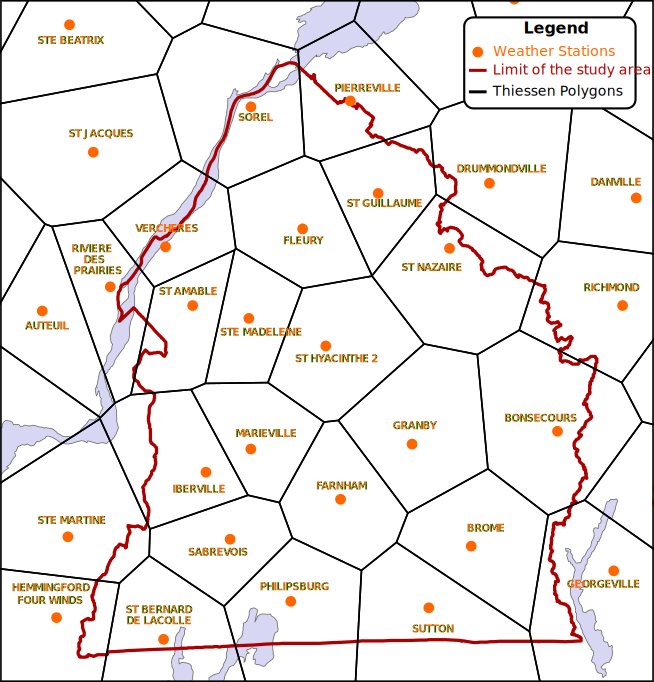
\includegraphics[width=0.75\textwidth]{img/Thiessen_meteo}
\caption[Locations of the weather stations in the Monteregie Est area.]{Locations of the weather stations in the Monteregie Est area.}
\label{fig:Thiessen_meteo}
\end{figure}


Tests have shown that inclusion of more than four stations does not significantly improve the interpolation and may in fact degrade the estimate. 

\subsection{Results and Discussion}

The quality of the estimates is strongly affected by seasonality. Stations at higher elevations are difficult to estimate accurately, in large part because of the topographical diversity of the surrounding stations leading to degradation of spatial coherence among stations.

The tendency for all of the methods to have a negative bias is indicative of the nature of precipitation distributions to be positively skewed (interpolated values will tend to cluster about the median error rather than the mean).

According to \cite{xia_forest_1999}, the two most important factors in climatology are the inter-correlations in the station network, and the seasonal variations in the relations between the stations.

\section{Future Work}

\end{document}